\documentclass[doc,natbib,12pt]{apa6}

\usepackage[american]{babel}
\usepackage[utf8x]{inputenc}
\usepackage{amsmath}
\usepackage{graphicx}
\usepackage[colorinlistoftodos]{todonotes}
\usepackage{varioref}
\usepackage[hidelinks]{hyperref}
\usepackage[T1]{fontenc}
\usepackage{listings}
\usepackage{color}
\usepackage{subcaption}

\definecolor{dkgreen}{rgb}{0,0.6,0}
\definecolor{gray}{rgb}{0.5,0.5,0.5}
\definecolor{mauve}{rgb}{0.58,0,0.82}

\lstset{frame=tb,
	language=Java,
	aboveskip=3mm,
	belowskip=3mm,
	showstringspaces=false,
	columns=flexible,
	basicstyle={\small\ttfamily},
	numbers=none,
	numberstyle=\tiny\color{gray},
	keywordstyle=\color{blue},
	commentstyle=\color{dkgreen},
	stringstyle=\color{mauve},
	breaklines=true,
	breakatwhitespace=true,
	tabsize=3
}
\title{Structure of the Pentium Microprocessor}
\shorttitle{Structure of the Pentium Microprocessor}
\author{Youwei Lu}
\affiliation{CISC 530-51- A-2018/Late Fall Assignment 2}

%\abstract{Referring to Operating Systems architecture, the topic of this assignment is on the ``Memory Management'' which is part of the computer's physical memory or Random-Access Memory (RAM) organization.}

\begin{document}
	\maketitle
	
	\section{Introduction}
	
	Pentium is a brand used for a series of x86 architecture-compatible microprocessors produced by Intel since 1993. Pentium processors are considered entry-level products that Intel rates as ``two stars'' \citep{Hesseldahl2000}, meaning that they are above the low-end Atom and Celeron series, but below the faster Core i3, i5, i7, i9, and high-end Xeon series.
	
	\subsection{Pentium Family}
	Intel first introduced microprocessors in 1969, with a 4-bit microprocessor 4004, then 8-bit microprocessors 8080 and 8085. Soon, 16-bit processors 8086 was introduced in 1979, which has 20-bit address bus and 16-bit data bus. 8088 is a less expensive version, which uses 8-bit data bus. Since then, the 80 series developed rapidly. 80186 in 1979, and 80286 was introduced in 1982, with 24-bit address bus, 16MB address space, enhanced with memory protection capabilities, and a protected mode was introduced. In 1985, the first 32-bit processor was invented: 80386. It supports 32-bit data bus and 32-bit address bus, 4GB address space, and introduced paging. An improved version 80486 was introduced in 1989.
	
	The time comes to 1993, and a new era arrived. Following their earlier naming conventions, Intel’s new fifth-generation chip was expected to be named the 586. However, Intel wanted to be able to register as a trademark the name of their new processor, and since numbers cannot be trademarked, the Pentium was born. Since this time the Pentium name has become one of the most widely recognized trademarks throughout the computer world. Intel announced its next generation of compatible microprocessors following the popular i486 CPU family. The design started in early 1989 with the primary goal of maximizing performance while preserving software compatibility within the practical constraints of available technology. The Pentium processor integrates 3.1 million transistors and carries the Intel trademark. \citep{Alpert1993}.
	
	Each processor in the Pentium series incorporates and builds off of the previous processor’s architectural achievements. \citep{Dandamudi2003} Pentium (80586) is similar to 486 but with a 64-bit data bus, and wider internal datapaths (128- and 256-bit wide), second execution pipeline added (to make superscalar performance and two instructions/clock), and doubled on-chip L1 cache. A branch prediction was also added. In 1995, Pentium Pro was introduced to carry three-way superscalar (3 instructions/clock), 36-bit address bus (so total is 64GB address space), and dynamic execution. In addition to the L1 cache, it has 256 KB L2 cache. With the commercial success of Pentium, Pentium II was introduced in 1997, and Pentium III in 1999, Pentium 4 in 2000. After that, Intel decides to use another brand name to make new generation microprocessors. For example, Itanium processor was the first one to use RISC design, instead of CISC.
	
	\subsection{Pentium Overview}
	\begin{figure}[htpb]
		\centering
		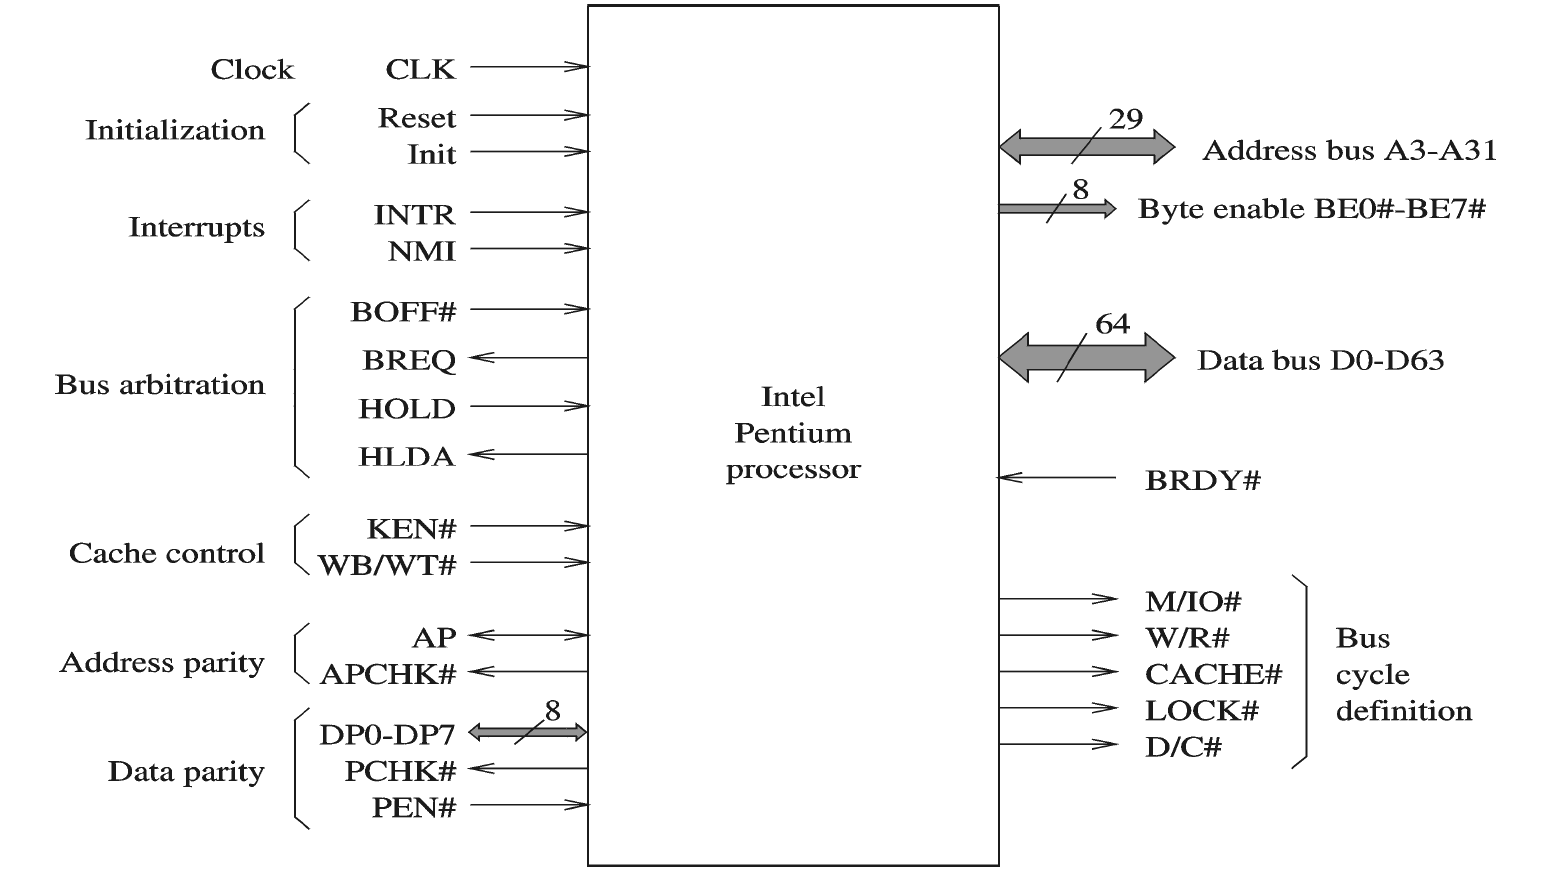
\includegraphics[width=1\textwidth]{overview.png}
		\caption{\label{fig:overview}A typical Pentium layout. \citep{Dandamudi2003}}
	\end{figure}
	A typical Pentium layout is shown in Figure~\vref{fig:overview}, and their addresses are explained below:
	\begin{itemize}
		\item Data bus (D0 - D63): 64-bit data bus.
		\item Address bus (A3 - A31): Only 29 lines, no A0-A2 (due to 8-byte wide data bus).
		\item Byte enables (BE0\# - BE7\#): Identifies the set of bytes to read or write. BE0\# specifies the least significant byte (D0 - D7), BE1\# specifies the next byte (D8 - D15), ... , BE7\# specifies the most significant byte (D56 - D63). Any combination of bytes can be specified.
		\item Data parity (DP0 - DP7): Even parity for 8 bytes of data. DP0 for D0 - D7, DP1 for D8 - D15, ... , DP7 for D56 - D63.
		\item Parity check (PCHK\#): Indicates the parity check result on data read. Parity is checked only for valid bytes, indicated by BE\# signals.
		\item Parity enables (PEN\#): Determines whether the parity check should be used.
		\item Address parity (AP): Bad address parity during inquire cycles.
		\item Memory/IO (M/IO\#): Defines bus cycle: memory or I/O.
		\item Write/Read (W/R\#): Distinguishes between write and read cycles.
		\item Data/Code (D/C\#): Distinguishes between data and code.
		\item Cacheability (CACHE\#):  Read cycle: indicates internal cacheability. Write cycle: burst write-back.
		\item Bus lock (LOCK\#): Used in a read-modify-write cycle. Useful in implementing semaphores.
		\item Interrupt (INTR): External interrupt signal.
		\item Nonmaskable interrupt (NMI): External NMI signal.
		\item Clock (CLK): System clock signal.
		\item Bus ready (BRDY\#): Used to extend the bus cycle. Introduces wait states.
		\item Bus request (BREQ): Used in bus arbitration.
		\item Backoff (BOFF\#): Aborts all pending bus cycles and floats the bus, useful to resolve the deadlock between two bus masters.
		\item Bus hold (HOLD): Completes outstanding bus cycles and floats bus. Asserts HLDA to give control of the bus to another master
		\item Bus hold acknowledges (HLDA): Indicates the Pentium has given control to another local master. Pentium continues execution from its internal caches.
		\item Cache enables (KEN\#): If asserted, the current cycle is transformed into cache line fill.
		\item Write-back/Write-through (WB/WT\#): Determines the cache write policy to be used.
		\item Reset (RESET): Resets the processor, starts execution at FFFFFFF0H. Invalidates all internal caches.
		\item Initialization (INIT): Similar to RESET but internal caches and FP registers are not flushed. After powerup, use RESET (not INIT)
	\end{itemize}
	
	\subsection{Pentium Structure}
	The Pentium processor is the successor to the Intel486 processor. Originally released with a 66MHz clock speed, it is a 16-bit based superscalar processor capable of executing two instructions in parallel during a single clock. It uses a CISC (Complex Instruction Set Computer) type instruction set and uses the little-endian type format to store bytes in memory. A 64-bit external bus, separate data, and instruction caches write buffers, and a pipelined floating-point unit combine to sustain a high executing rate. Caching along with pipeline and instruction flow are discussed in detail in this article. 
	
	A Pentium processor’s major functional components are: \citep{pctechguide}
	\begin{itemize}
		\item Core: The heart of a Pentium is the execution unit. The Pentium has two parallel integer pipelines enabling it to read, interpret, execute and despatch two instructions simultaneously.
		\item Branch Predictor: The branch prediction unit tries to guess which sequence will be executed each time the program contains a conditional jump, so that the Prefetch and Decode Unit can get the instructions ready in advance.
		\item Floating Point Unit: The third execution unit in a Pentium, where non-integer calculations are performed.
		\item Level 1 Cache: The Pentium has two on-chip caches of 8KB each, one for code and one for data, which are far quicker than the larger external secondary cache.
		\item Bus Interface: This brings a mixture of code and data into the CPU, separates the two ready for use, and then recombines them and sends them back out.
	\end{itemize}
	
	\begin{figure}[htpb]
		\centering
		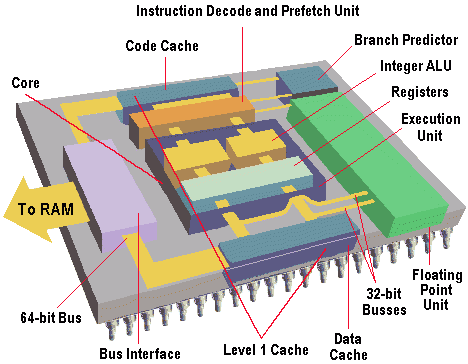
\includegraphics[width=1\textwidth]{21proc.png}
		\caption{\label{fig:structure}Basic Structure of a Pentium Microprocessor. \citep{pctechguide}}
	\end{figure}
	
	
	All the elements of the processor stay in step by use of a clock which dictates how fast it operates. The very first microprocessor had a 100KHz clock, whereas the Pentium Pro uses a 200MHz clock, which is to say it ticks 200 million times per second. As the clock ticks, various things happen. The Program Counter (PC) is an internal memory location which contains the address of the next instruction to be executed. When the time comes for it to be executed, the Control Unit transfers the instruction from memory into its Instruction Register (IR). \citep{pctechguide}
	
	At the same time, the PC is incremented so that it points to the next instruction in sequence; now the processor executes the instruction in the IR. Some instructions are handled by the Control Unit itself, so if the instruction says jump to location 2749, the value of 2749 is written to the PC so that the processor executes that instruction next. \citep{pctechguide}
	
	Many instructions involve the arithmetic and logic unit (ALU). This works in conjunction with the General Purpose Registers – temporary storage areas which can be loaded from memory or written to memory. A typical ALU instruction might be to add the contents of a memory location to a general purpose register. The ALU also alters the bits in the Status Register (SR) as each instruction is executed; this holds information on the result of the previous instruction. Typically, the SR has bits to indicate a zero result, an overflow, a carry and so forth. The control unit uses the information in the SR to execute conditional instructions such as jump to address 7410 if the previous instruction overflowed. \citep{pctechguide}
	
	The following of this paper will introduce some basic topics about microprocessors, with special emphasize on Pentium. The concepts of basic of computer architecture will first be introduced on page~\pageref{chp:computerArchitecture}, then the branch prediction is introduced on page~\pageref{chp:branchPrediction}, and the system architecture is discussed on page~\pageref{chp:systemArchitecture}. Some advanced technologies should be studied, as rapid execution module on page~\pageref{chp:rapidExecutionModule}, memory subsystem on page~\pageref{chp:memorySubsystem}, and hyperthreading technology on page~\pageref{chp:hyperthreadingTechnology}. As we know, Pentium uses CISC, not RISC. Their differences are introduced and compared on page~\pageref{chp:RISCvsCISC}.
	
	As a summary and page reference, a complete explanation is given for the following issues:
	
	\begin{itemize}
		
		
		\item   Concepts of Computer Architecture. (page~\pageref{chp:computerArchitecture})
		
		
		\item   Branch Prediction. (page~\pageref{chp:branchPrediction})
		
		\item   System Architecture. (page~\pageref{chp:systemArchitecture})
		
		\item   Rapid Execution Module. (page~\pageref{chp:rapidExecutionModule})
		
		\item   Memory Subsystem. (page~\pageref{chp:memorySubsystem})
		
		\item   Hyperthreading Technology. (page~\pageref{chp:hyperthreadingTechnology})
		
		\item   RISC and CISC Convergence, Advantages of RISC, Design Issues of RISC Processors. (page~\pageref{chp:RISCvsCISC})
		
	\end{itemize}
	
	
	
	\newpage
	\section{Concepts of Computer Architecture} \label{chp:computerArchitecture}
	
	In a programmer's view, the computer architecture is a structure of a computer that a machine language programmer must understand to write a correct (timing independent) program for the machine. The computer architecture is a set of rules that explain the functionality, organization, and implementation of computer systems. \citep{Shrestha2014}
	
	One concept that people often get confused is the computer organization. It is actually from the implementer's view, which refers to the actual hardware structure and realization. Table.~\vref{tab:compare} gives a comparison of Computer Architecture and Computer Organization.
	
	\begin{table}[htpb]
		\centering
		\begin{tabular}{p{2in}|p{2in}}
			Computer Architecture & Computer Organization \\\hline
			Computer architecture is concerned with the structure and behavior of computer systems as seen by the user. & computer organization is concerned with the way the hardware components operate and the way they are connected together to form a computer system. \\
			It includes information, formats, instruction set, and techniques for addressing memory. & It includes hardware details transparent to the programmer such as control signal and peripheral. \\
			It describes what the computer does. & It describes how the computer performs. Ex, circuit design, control signals, memory types and etc.
		\end{tabular}
		\caption{\label{tab:compare}Computer Architecture vs Computer Organization. \citep{Shrestha2014}}
	\end{table}
	
	There are usually 6 layers of computer architecture, as shown in Figure.~\vref{fig:layers}:
	\begin{figure}[htpb]
		\centering
		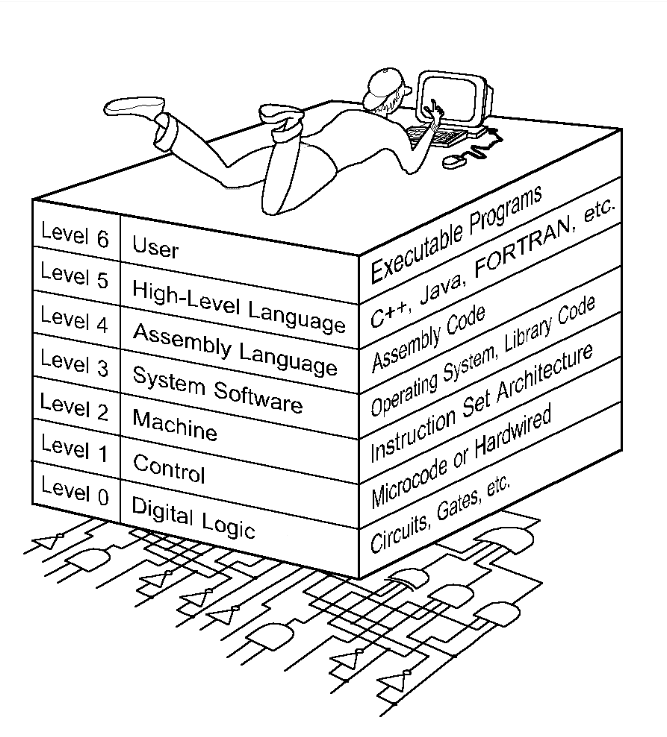
\includegraphics[width=1\textwidth]{C1.png}
		\caption{\label{fig:layers}Computer Architecture Layers \citep{Null2012}}
	\end{figure}
	Each level is an abstraction of the level below it. The machines at each level execute their own particular instructions, calling upon machines at lower levels to perform tasks as required. All the work is ultimately carried out by computer circuits. \citep{Null2012}.
	
	In the first computer, ENIAC, all programming was done at the digital logic level, and a different hardware configuration was needed to solve every unique problem type. John von Neumann invented the computer that could store instructions in memory. These stored-program computers have become known as von Neumann Architecture systems.
	
	\begin{figure}[htpb]
		\centering
		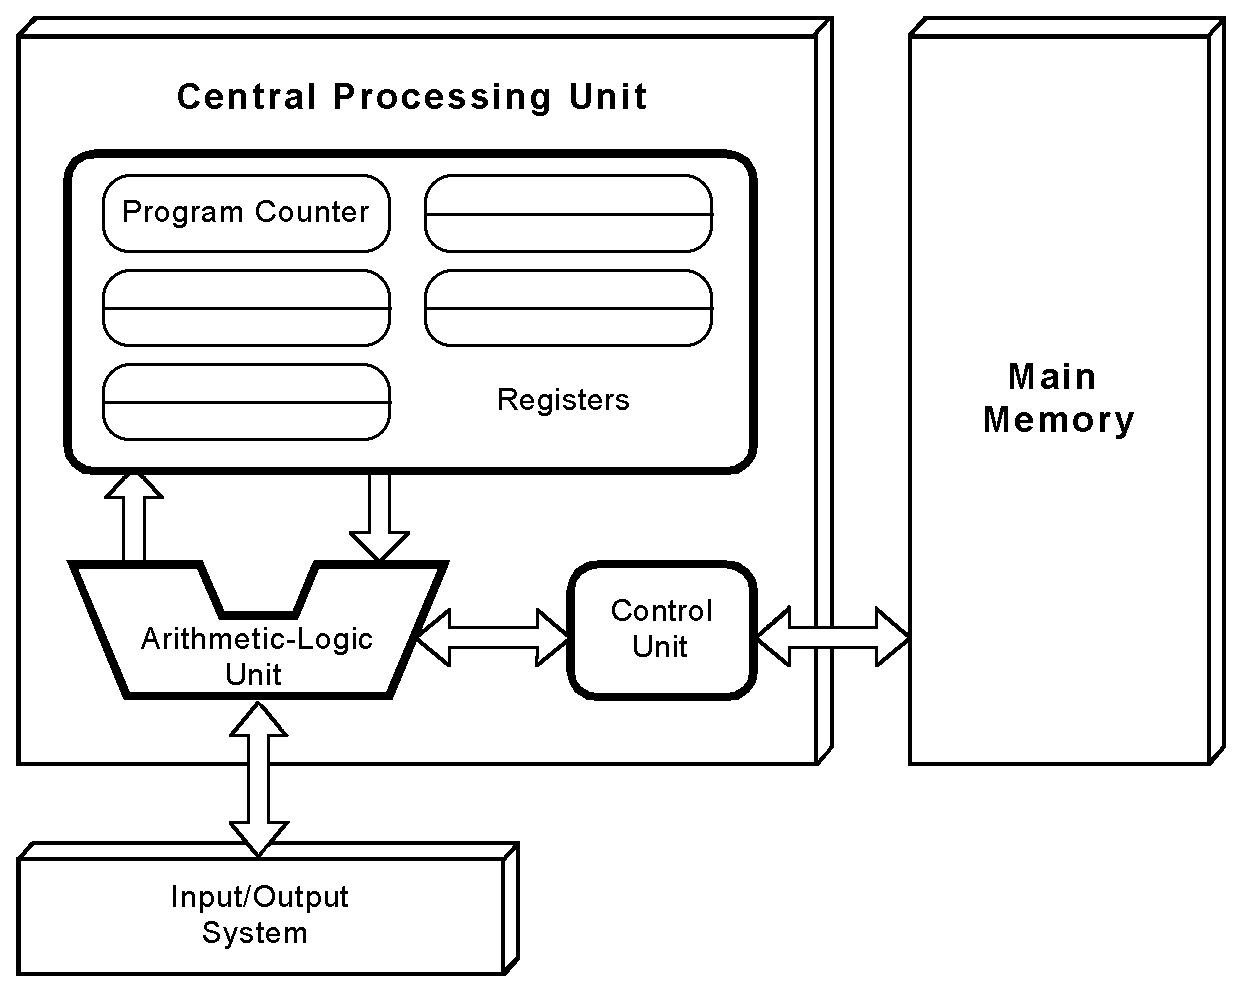
\includegraphics[width=1\textwidth]{von.png}
		\caption{\label{fig:von}The von Neumann Model \citep{Null2012}}
	\end{figure}
	
	Today's stored-program computers have the following characteristics as shown in Figure.~\vref{fig:von}:
	\begin{itemize}
		\item Three hardware systems: A central processing unit (CPU), The main memory system, and An i/O system
		\item the capacity to carry out sequential instruction processing
		\item A single data path between the CPU and main memory (known as von Neumann bottleneck)
	\end{itemize}
	
	In a von Neumann model, digital computation in ALU Internal storage of data is programmable via a standard set of instructions, with internal storage of program input/output. It has automatic sequencing of instruction execution (by control mechanism).
	
	\subsection{Pentium Improvements on von Neumann}
	Conventional stored-program von Neumann computers have undergone many incremental improvements over the years, especially with the help from Intel. These improvements include adding processors, specialized buses, floating-point units, and cache memories. Adding processors is a typical and most significant way to improve von Neumann architecture, and Pentium started to manufacture multi-core processors since Pentium D.
	
	The Pentium D brand refers to two series of desktop dual-core 64-bit x86-64 microprocessors with the NetBurst microarchitecture, which is the dual-core variant of Pentium 4 ``Prescott'' manufactured by Intel. Each CPU comprised two dies, each containing a single core, residing next to each other on a multi-chip module package. The brand's first processor, codenamed Smithfield, was released by Intel on May 25, 2005. \citep{Intel2007}.
	
	\newpage
	\section{Branch Prediction} \label{chp:branchPrediction}
	
	Branch prediction is one of the ancient performance improving techniques which still finds relevance to modern architectures. To understand the motivation for branch prediction, we first need to know how instruction is executed.
	
	Each instruction includes fetch, decode, execute, and write-back stages. When waiting in a branch (e.g. an if-then-else structure), the pipeline is waiting for the result for the next step. Figure.~\vref{fig:pipeline} shows an example of a 4-stage pipeline. The colored boxes represent instructions independent of each other. Modern processors may have more than 10 pipeline stages between next PC calculation and branch resolution, and you can imagine how much work is lost if the pipeline doesn't follow correct instruction flow.
	
	\begin{figure}[htpb]
		\centering
		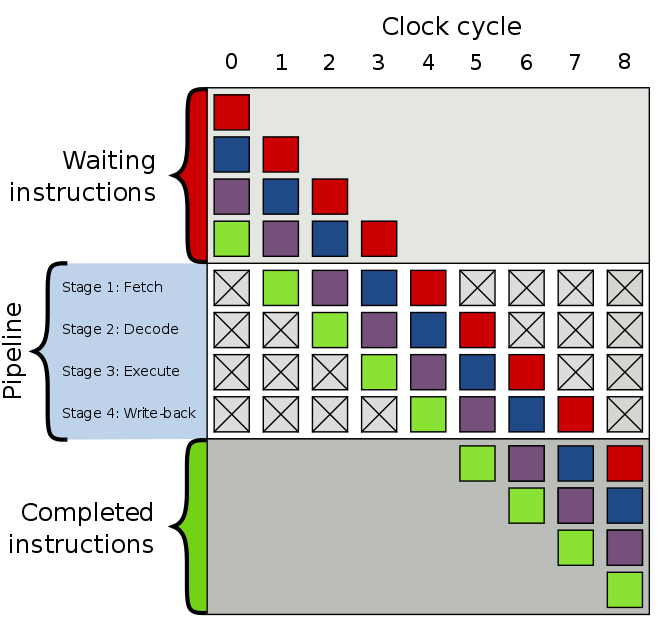
\includegraphics[width=0.6\textwidth]{660px-Pipeline.png}
		\caption{\label{fig:pipeline}Example of 4-stage pipeline. \citep{Kolinko}}
	\end{figure}
	
	Therefore, as branch penalties limit the performance of deeply pipelined processors, modern branch predictors are used to providing high accuracy and can reduce branch penalties.
	
	Without branch prediction, the processor would have to wait until the conditional jump instruction has passed the execute stage before the next instruction can enter the fetch stage in the pipeline. Prediction works by executing instructions from both paths of the branch and only permitting those instructions from the taken path to modify architectural state. \citep{Vinyard2000}
	
	\citep{Vinyard2000} also presents a very good example as below:
	
	Given the following source code:
	\begin{lstlisting}
	if (emp_status == ACTIVE) {
	n_active_emps++;
	total_payroll += emp_pay;
	}
	else {
	n_inactive_emps++;
	}
	\end{lstlisting}
	This code is typically complied into a sequence such as:
	\begin{lstlisting}
	{
	cmp.ne p1 = rs, ACTIVE   // compare emp_status
	(p1) br else             // jump to else code if condition fails
	}
	.label then
	{
	add  rt = rt, rp         // sum total_payroll + emp_pay
	add  ra = ra, 1          // increment n_active_emps
	br  join
	}
	.label else
	{
	add  ri = ri, 1          // increment n_inactive_emps
	}
	.label join
	\end{lstlisting}
	The generated predicted code would look like:
	\begin{lstlisting}
	{
	cmp.eq  p1, p2 = rs, ACTIVE  // compare emp_status
	} 
	{
	(p1)  add rt = rt, rp        // sum total_payroll + emp_pay
	(p1)  add ra = ra, 1         // increment n_active_emps
	(p2)  add ri = ri, 1         // increment n_inactive_emps
	}
	\end{lstlisting}
	
	In the above example, it is very clear that the three predicted instructions can be executed in parallel. Each of the instructions above is predicted. If the instruction's predicate evaluates to a 1, the instruction is executed. Otherwise, the instruction equates to a NOP. On a machine with three or more additional units, the above example utilizes the same cycles as a non-predicated machine except there is no possibility of a branch penalty. \citep{Vinyard2000}
	
	An even more clear diagram can be found in \citep{Byte} as shown in Figure.~\vref{fig:prediction}.
	
	\begin{figure}[htpb]
		\centering
		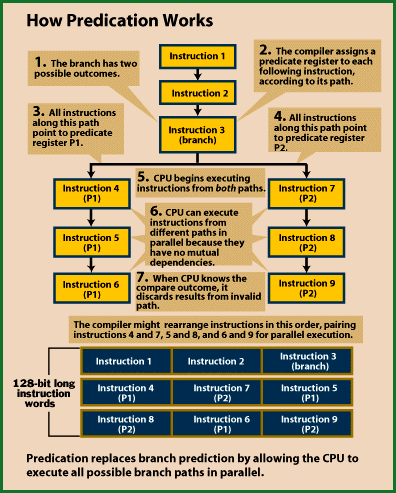
\includegraphics[width=1\textwidth]{how_Predication_Works-Byte.png}
		\caption{\label{fig:prediction}How Prediction Works. \citep{Byte}}
	\end{figure}
	
	There are typically two kinds of branch prediction: Static Branch Prediction and Dynamic Branch Prediction.
	
	\subsection{Static Branch Prediction}
	Static Branch Prediction predicts always the same direction for the same branch during the whole program execution.
	It comprises hardware-fixed prediction and compiler-directed prediction.
	Simple hardware-fixed direction mechanisms can be:
	\begin{itemize}
		\item Predict always not taken
		\item Predict always taken
		\item Backward branch predict taken, forward branch predict not taken
	\end{itemize}
	
	Sometimes a bit in the branch opcode allows the compiler to decide the prediction direction. \citep{McFarland2006}
	
	\subsection{Dynamic Branch Prediction}
	Dynamic Branch Prediction: the hardware influences the prediction while execution proceeds.
	Prediction is decided on the computation history of the program.
	During the start-up phase of the program execution, where a static branch prediction might be effective, the history information is gathered and dynamic branch prediction gets effective.
	In general, dynamic branch prediction gives better results than static branch prediction, but at the cost of increased hardware complexity. \citep{McFarland2006}
	
	Usually, Dynamic Branch Prediction improve performance and reduce energy by decreasing the number of instructions executed on the wrong path.
	However, reducing latency and storage overhead of BP while maintaining high accuracy presents significant challenges. A survey of dynamic branch prediction techniques can be found in \citep{Mittal2016}.
	
	
	\subsection{Pentium on Branch Prediction}
	Pentium uses Dynamic Branch Prediction. 
	
	It is implemented using 4 way set associated cache with 256 entries. This is called Branch Target Buffer (BTB). The directory entry for each line consists of:
	\begin{itemize}
		\item Valid bit: indicates whether the entry is valid or not.
		\item History bit: Track how often bit has been taken.
	\end{itemize}
	
	Their four states can be illustrated in the diagram Figure.~\vref{fig:BTB}
	\begin{figure}[htpb]
		\centering
		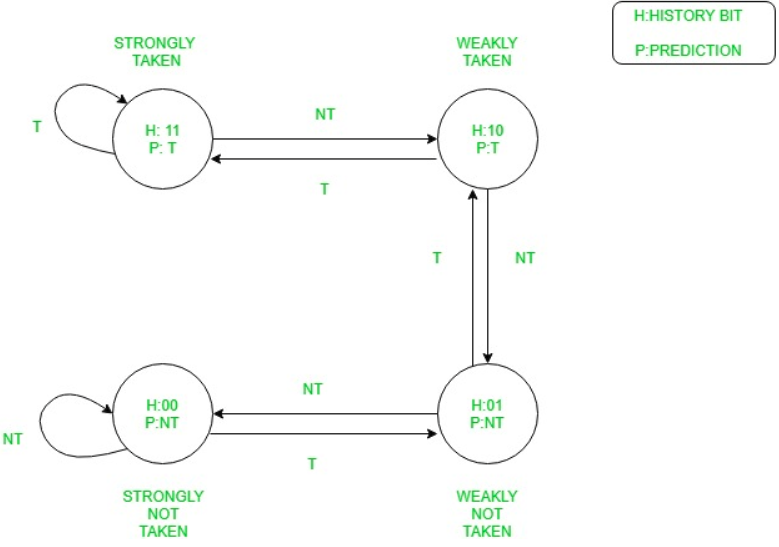
\includegraphics[width=1\textwidth]{222-15.png}
		\caption{\label{fig:BTB}4 Stage way. \citep{GeeksforGeeks}}
	\end{figure}
	and explained by the table:
	
	\begin{table}[htpb]
		\centering
		\begin{tabular}{p{1in}|p{1in}|p{1in}|p{1in}|p{1in}}
			History Bits & Resulting Description & Prediction Made & If Branch Taken & If Branch Not Taken \\\hline
			11    & Strongly Taken &    Branch Taken    & Remains in same state    & Downgraded to weakly taken \\
			10 &    Weakly Taken &    Branch Taken &    Upgraded to strongly taken &    Downgraded to weakly not taken \\
			01    & Weakly Not Taken &    Branch Not Taken &    Upgraded to weakly taken &    Downgraded to strongly not taken \\
			00    & Strongly Not Taken &     Branch Not Taken &    Upgraded to weakly & not taken    Remains in same state
		\end{tabular}
		\caption{\label{tab:BTB}4 Stage way. }
	\end{table}
	
	
	
	\newpage
	\section{System Architecture} \label{chp:systemArchitecture}
	
	The system architecture was partly discussed in the section on page~\pageref{chp:computerArchitecture}, and we already understand the architecture of a von Neumann computer, as clearly shown in Fig.~\vref{fig:von}, I'd like to take the chance to focus on Pentium structure in this section.
	
	\subsection{Pentium Architecture}
	
	The first Pentium processors were introduced in 1993. It runs at a clock frequency of either 60 or 66 MHz and has 3.1 million transistors. Some of the features of Pentium architecture are \citep{Das}
	
	\begin{itemize}
		\item Complex Instruction Set Computer (CISC) architecture with Reduced Instruction Set Computer (RISC) performance.
		\item 64-Bit Bus.
		\item Upward code compatibility.
		\item Pentium processor uses Superscalar architecture and hence can issue multiple instructions per cycle.
		\item Multiple Instruction Issue (MII) capability.
		\item Pentium processor executes instructions in five stages. This staging, or pipelining, allows the processor to overlap multiple instructions so that it takes less time to execute two instructions in a row.
		\item The Pentium processor fetches the branch target instruction before it executes the branch instruction.
		\item The Pentium processor has two separate 8-kilobyte (KB) caches on a chip, one for instructions and one for data. It allows the Pentium processor to fetch data and instructions from the cache simultaneously.
		\item When data is modified, only the data in the cache is changed. Memory data is changed only when the Pentium processor replaces the modified data in the cache with a different set of data.
		\item The Pentium processor has been optimized to run critical instructions in fewer clock cycles than the 80486 processor.
	\end{itemize}
	
	\begin{figure}[htpb]
		\centering
		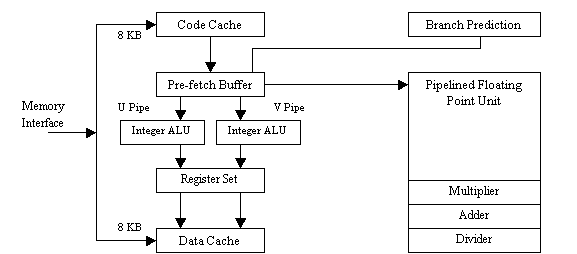
\includegraphics[width=1\textwidth]{1.png}
		\caption{\label{fig:superscalar}Superscalar Architecture of Pentium. \citep{Das}}
	\end{figure}
	
	The Pentium processor has two primary operating modes: \citep{Das}
	\begin{itemize}
		\item Protected Mode - In this mode all instructions and architectural features are available, providing the highest performance and capability. This is the recommended mode that all new applications and operating systems should target.
		\item Real-Address Mode - This mode provides the programming environment of the Intel 8086 processor, with a few extensions. Reset initialization places the processor in real mode where, with a single instruction, it can switch to protected mode.
	\end{itemize}
	
	\newpage
	\section{Rapid Execution Module} \label{chp:rapidExecutionModule}
	The Rapid Execution Module was introduced to the market by Intel and given a more beautiful commercial name: NetBURST. Using Rapid Execution Engine certain instructions may be executed at twice the normal speed.
	
	A pipeline is an execution unit which takes in decoded micro-instructions. The X86 instructions are first decoded and then sent to the pipeline. The longer the pipeline is, the quicker an instruction can be executed. Each stage executes a minor part of the work and by spreading the work on "more hands", the efficiency is increased.\citep{Karbosguide}
	
	
	\begin{figure}[htpb]
		\centering
		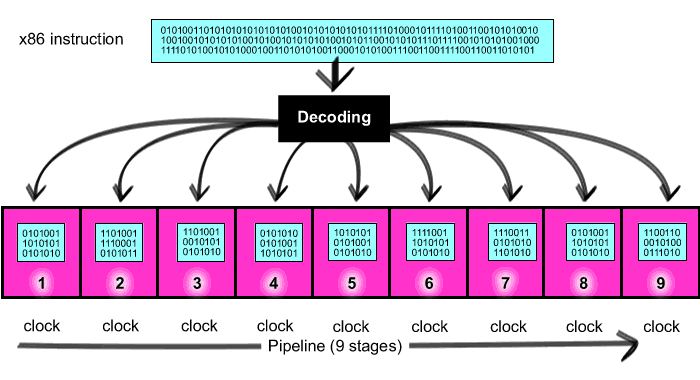
\includegraphics[width=1\textwidth]{_775.png}
		\caption{\label{fig:20stage}Stages of pipeline. \citep{Karbosguide}}
	\end{figure}
	
	In Pentium III the pipeline was of 10 stages. In Pentium 4 it has been increased to 20 stages.
	
	The problem with the long pipeline is, that it takes to a long time load the instruction. And if the instruction should not have been loaded at all, the error is most costly (in time) the longer the pipeline becomes. \citep{Karbosguide}
	
	With many instructions being executed simultaneously you cannot avoid loading the wrong instruction (called misprediction) from time to time. And a shorter pipeline is quicker to recover this error - fewer stages have to be cleared and reloaded. \citep{Karbosguide}
	
	The benefit from a pipeline increased from 10 stages to 20, is to open up for new higher clock frequencies. When each instruction is executed in more stages, it can be done a lot quicker. \citep{Karbosguide}
	
	
	\newpage
	\section{Memory Subsystem} \label{chp:memorySubsystem}
	
	In a user(or even programmer)'s view, the computer memory is flat, large storage space. However, this is not possible with current technology. We wanna the fastest computer, so we can make fast memories by using static RAM, but its speed drops as the memory size increases. At the same time, Dynamic RAM can be used for slow but large memory space. 
	
	Generally, fast storage technologies cost more per byte, have less capacity, and require more power (heat!). To balance performance and cost, computer memory systems typically consist of a four-level hierarchy: Registers — Cache — Main Memory — Backing Store (i.e. disk). Note that data is moved between the cache, main memory, and backing store transparently, but data movement between registers and the rest of memory is explicitly under the control of the program. It is up to the compiler to decide which data items should be moved to registers, and when, and the compiler must compile into the code the relevant load and store instructions. \citep{Stevens2009}
	
	In practice, many computers introduce another level into the hierarchy: they have two levels of cache; a small (perhaps 64Kbyte), very fast cache on the processor chip (called the first level cache), and a larger (perhaps 512Kbyte) second level cache, either on the processor chip or on separate chips, and intermediate in speed between the on-chip cache and the main memory. \citep{Stevens2009}
	
	
	\begin{figure} [htpb]
		\centering
		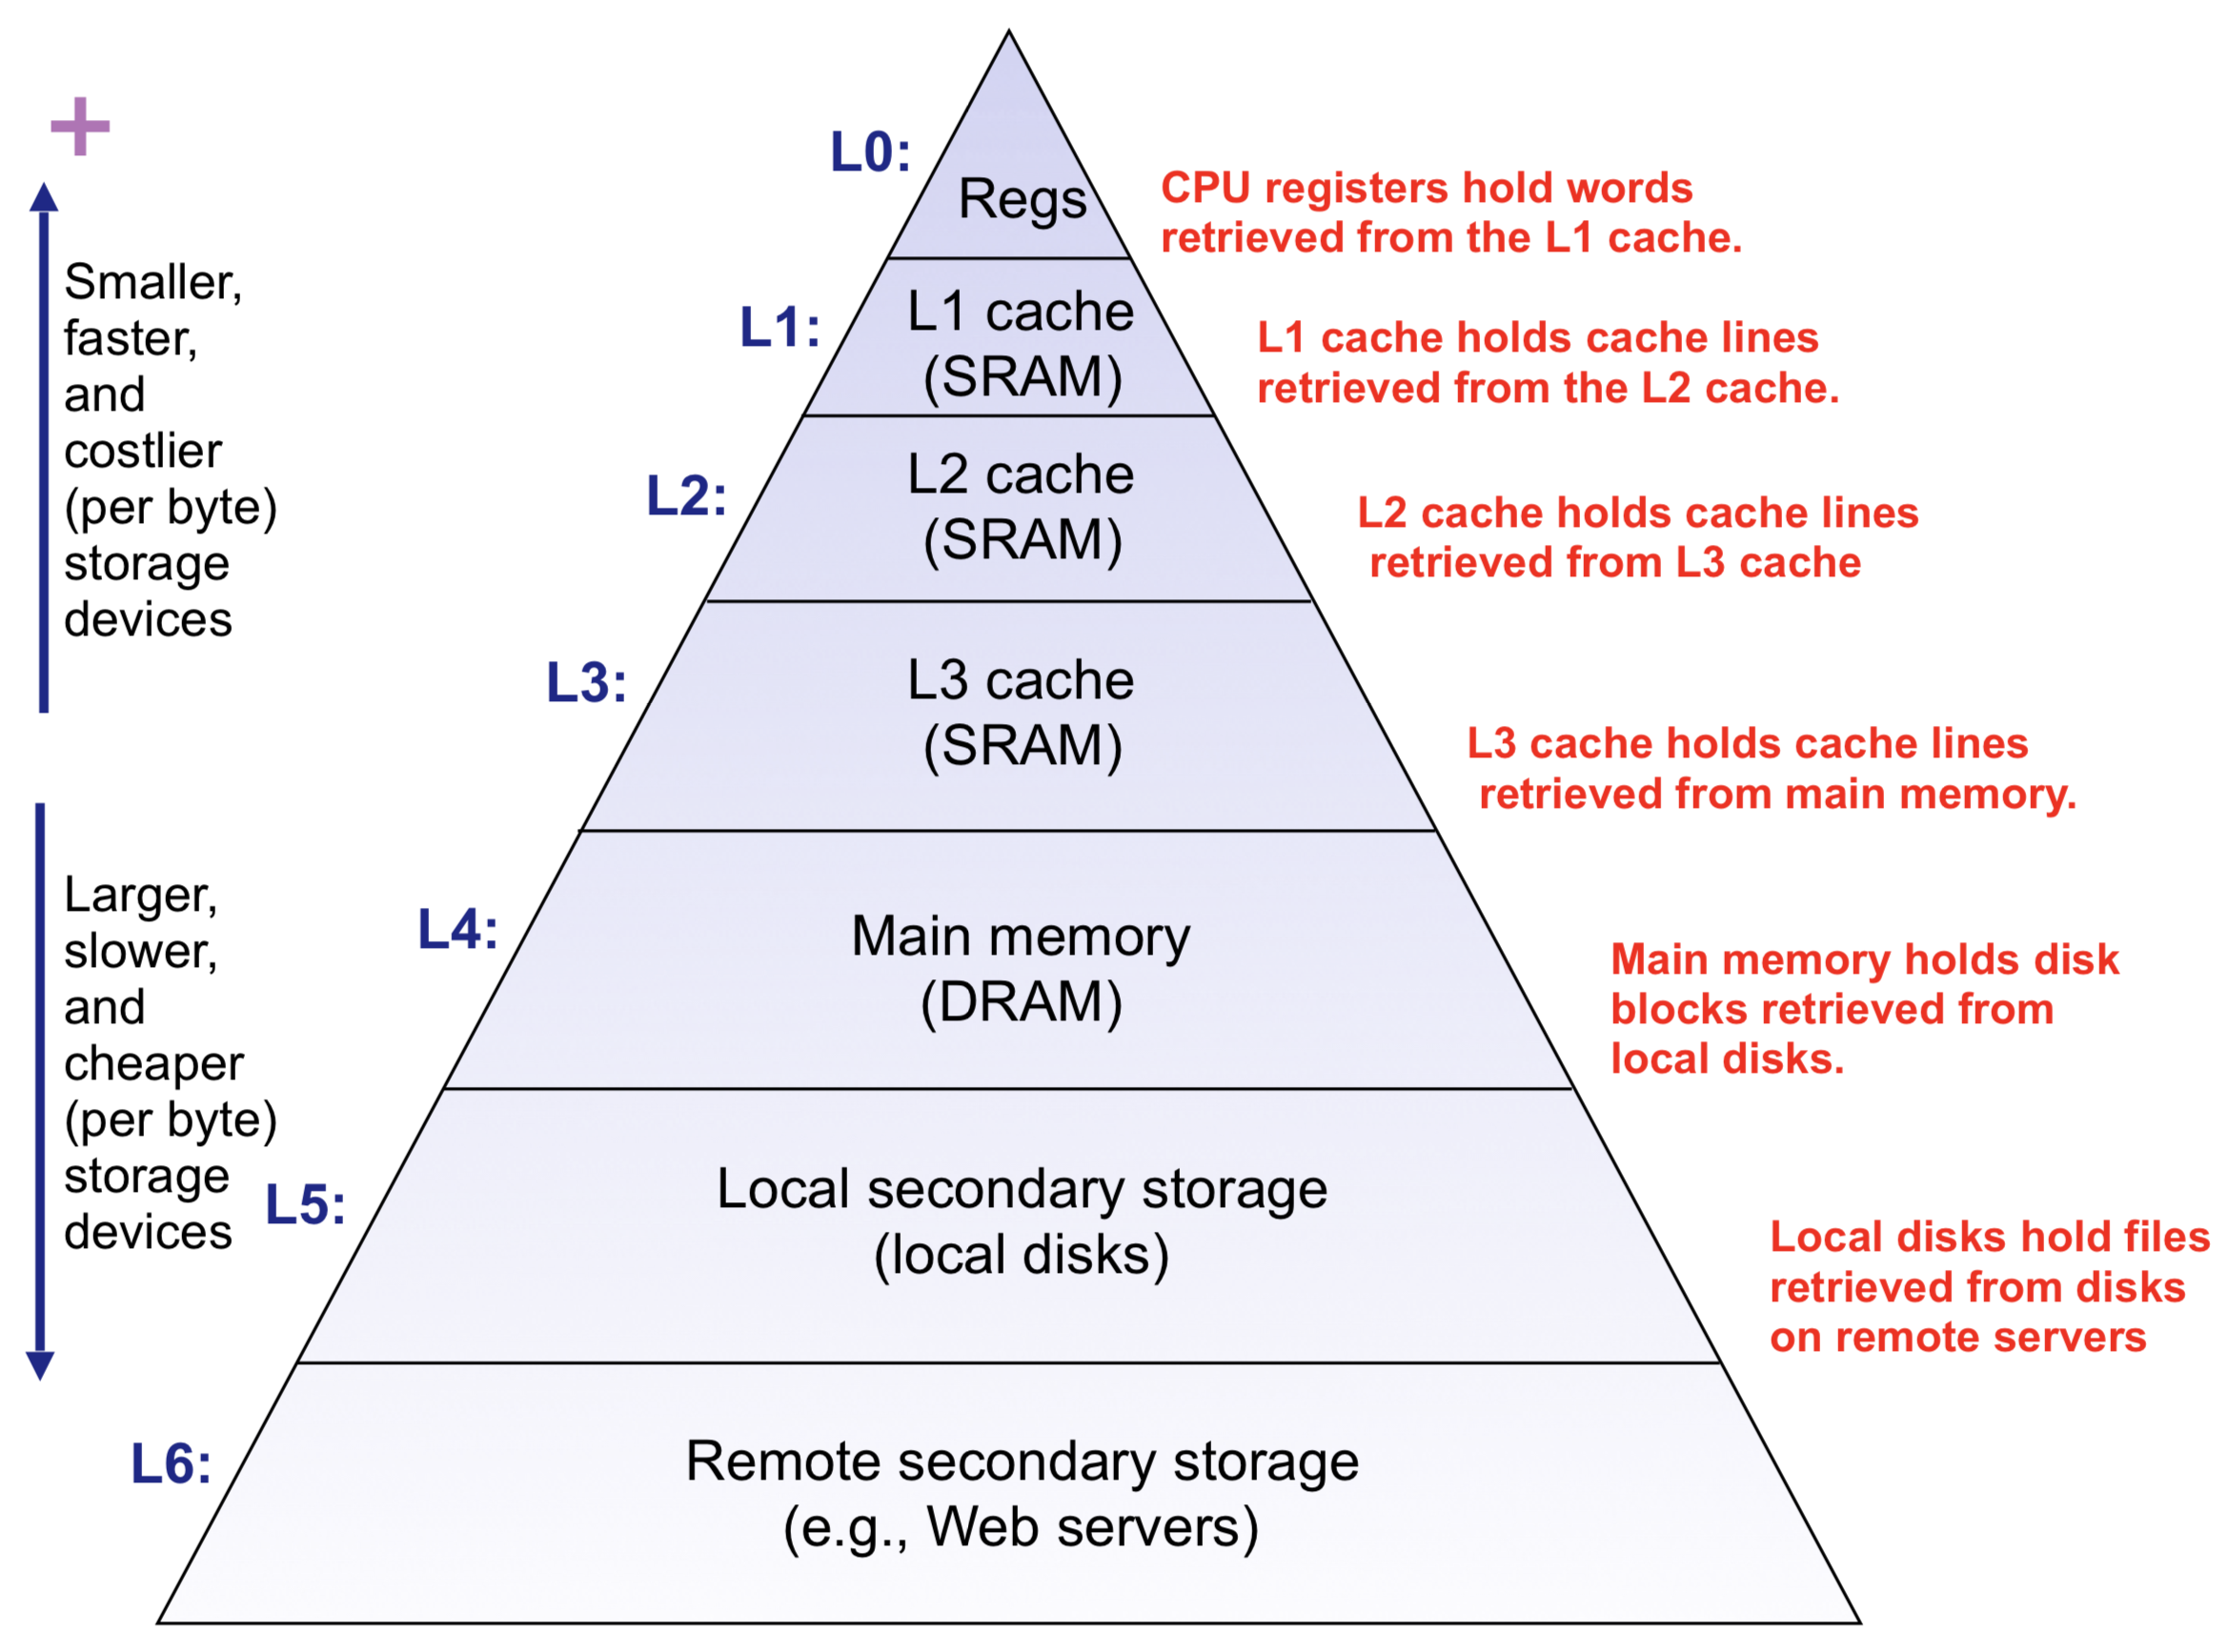
\includegraphics[width=0.8\textwidth]{subsytems.png}
		\caption{\label{fig:subsytems}Memory Hierarchy \citep{Bryant2015}}
	\end{figure}    
	
	One can refer to Figure.~\vref{fig:subsytems} for a complete list of the memory hierarchy. 
	
	\subsection{Pentium Memory Subsystem}
	
	\begin{figure}
		\centering
		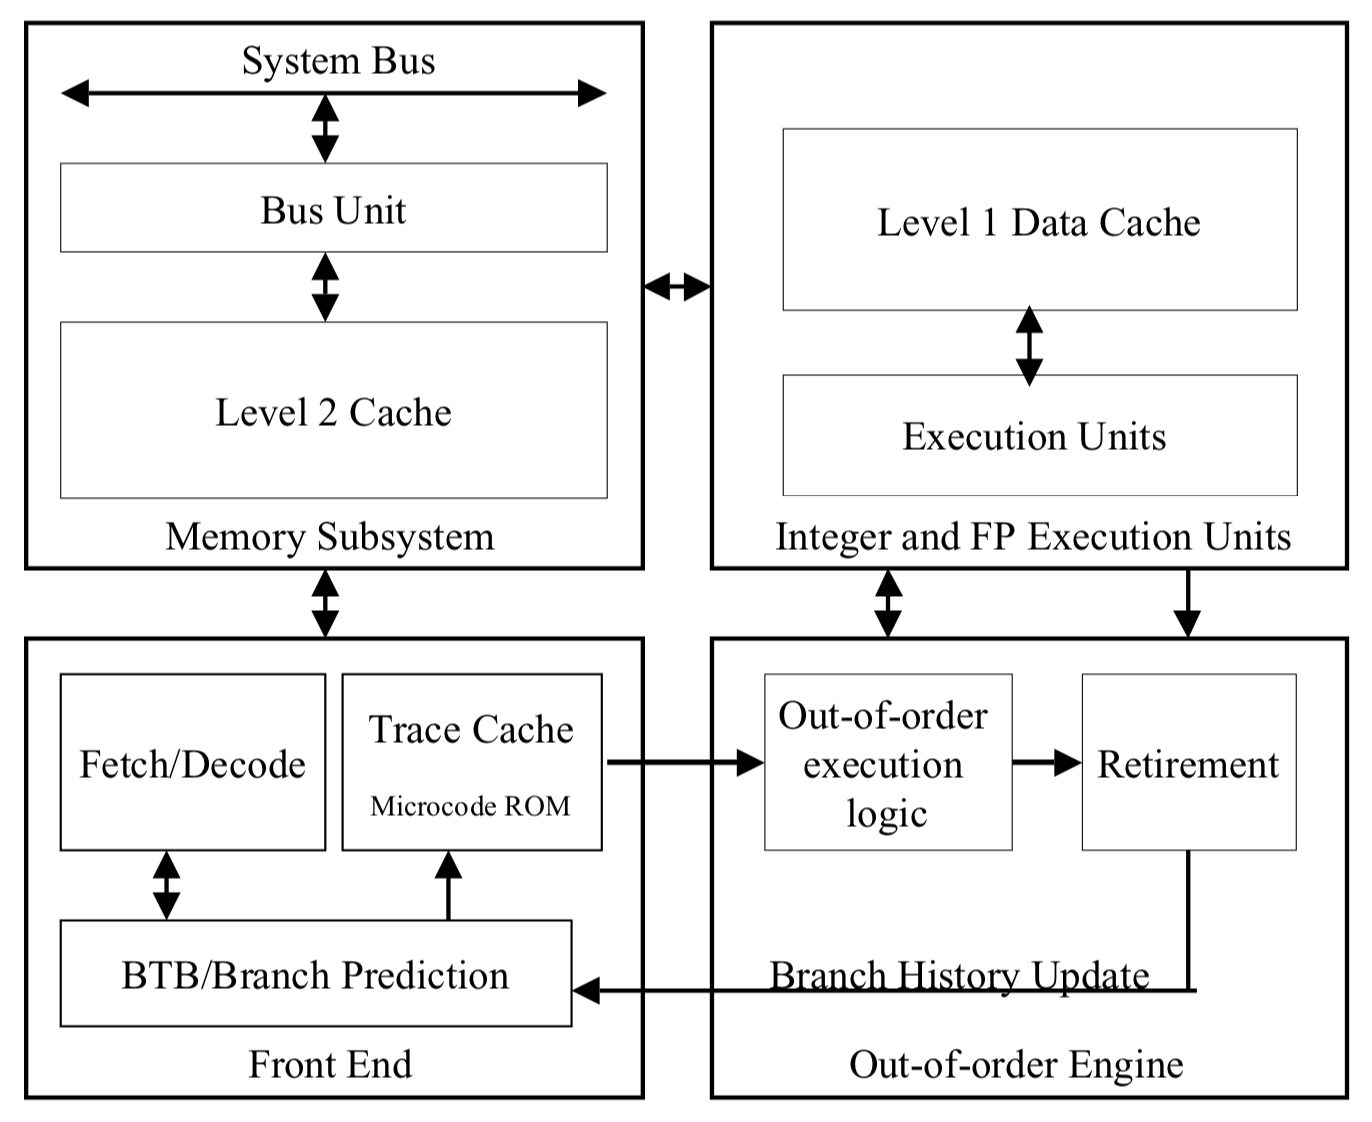
\includegraphics[width=0.8\textwidth]{pentiumMemory.png}
		\caption{\label{fig:pentiumMemory}Pentium Memory Hierarchy \citep{Hinton2001}}
	\end{figure}    
	
	
	
	Figure.~\vref{fig:pentiumMemory} shows the memory subsystem of Pentium. This includes the L2 cache and the system bus. The L2 cache stores both instructions and data that cannot fit in the Execution Trace Cache and the L1 data cache. The external system bus is connected to the backside of the second-level cache and is used to access main memory when the L2 cache has a cache miss, and to access the system I/O resources. \citep{Hinton2001}
	
	
	
	
	
	\newpage
	\section{Hyperthreading Technology} \label{chp:hyperthreadingTechnology}
	
	Hyperthreading technology is a process that allows an Intel Pentium 4 CPU to be viewed by the operating systems as two processors. From a software or architecture perspective, this means operating systems and user programs can schedule processes or threads to logical processors as they would on multiple physical processors. From a microarchitecture perspective, this means that instructions from both logical processors will persist and execute simultaneously on shared execution resources. \citep{Marr2002}
	
	To make the physical processor appear as multiple logical processors, there is one copy of the architecture state for each logical processor, and the logical processors share a single set of physical execution resources. From a software or architecture perspective, this means operating systems and user programs can schedule processes or threads to logical processors as they would on conventional physical processors in a multiprocessor system. From a microarchitecture perspective, this means that instructions from logical processors will persist and execute simultaneously on shared execution resources. \citep{Marr2002}
	
	\begin{figure} [htpb]
		\centering
		\begin{subfigure}{.45\textwidth}
			\centering
			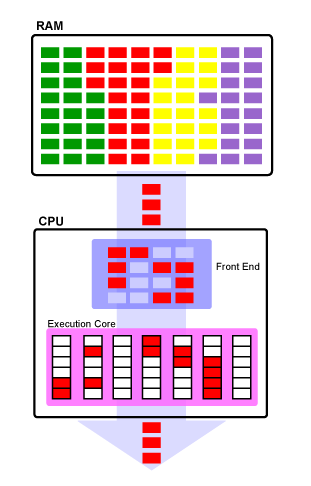
\includegraphics[width=1\linewidth]{single_thread-single_cpu.png}
			\caption{Single-threaded CPU. \citep{Stokes2002}}
			\label{fig:single_thread-single_cpu}
		\end{subfigure}%
		\begin{subfigure}{.45\textwidth}
			\centering
			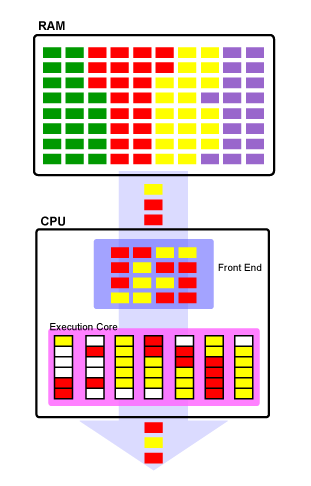
\includegraphics[width=1\linewidth]{hyperthread-single_cpu.png}
			\caption{Hyper-threaded CPU. \citep{Stokes2002}}
			\label{fig:hyperthread-single_cpu}
		\end{subfigure}
		\caption{Comparison of single and hyperthreading CPU}
		\label{fig:test}
	\end{figure}
	
	To clearly show the improvement, we may compare the front-end behavior in CPU. The front end of the pipeline is responsible for delivering instructions to the later pipe stages.
	
	In Figure.~\vref{fig:single_thread-single_cpu}, the different colored boxes in RAM represent instructions for four different running programs. As you can see, only the instructions for the red program are actually being executed right now. \citep{Stokes2002} 
	
	In comparison, Figure.~\vref{fig:hyperthread-single_cpu} illustrates that super-threading has all instructions issued by the front end on each clock from the same thread.
	
	
	
	\newpage
	\section{RISC and CISC Convergence, Advantages of RISC, Design Issues of RISC Processors} \label{chp:RISCvsCISC} 
	
	CISC stands for ``Complex Instruction Set Computer'', and RISC stands for ``Reduced Instruction Set Computer''. CISC systems try to improve performance by reducing the number of instructions per program. In contrary, RISC system shortens execution time by reducing the clock cycles per instruction. 
	
	\subsection{RISC}
	
	Advantages of RISC processor architecture:  \citep{elprocus}
	\begin{itemize}
		\item Because of the small set of instructions of RISC, high-level language compilers can produce more efficient code.
		\item RISC allows freedom of using the space on microprocessors because of its simplicity.
		Instead of using Stack, many RISC processors use the registers for passing arguments and holding the local variables.
		\item RISC functions use only a few parameters, and the RISC processors cannot use the call instructions, and therefore, use fixed length instructions which are easy to pipeline.
		\item The speed of the operation can be maximized and the execution time can be minimized.
		\item Very less number of instruction formats (less than four), a few numbers of instructions (around 150) and a few addressing modes (less than four) are needed.
	\end{itemize}
	
	Drawbacks of RISC processor architecture: \citep{elprocus}
	\begin{itemize}
		\item With the increase in the length of the instructions, the complexity increases for the RISC processors to execute due to its character cycle per instruction.
		\item The performance of the RISC processors depends mostly on the compiler or programmer as the knowledge of the compiler plays a major role while converting the CISC code to a RISC code; hence, the quality of the generated code depends on the compiler.
		\item While rescheduling the CISC code to a RISC code, termed as a code expansion, will increase the size. And, the quality of this code expansion will again depend on the compiler, and also on the machine’s instruction set.
		\item The first level cache of the RISC processors is also a disadvantage of the RISC, in which these processors have large memory caches on the chip itself. For feeding the instructions, they require very fast memory systems.
	\end{itemize}
	
	\subsection{CISC}
	
	Advantages of CISC architecture: \citep{elprocus}
	\begin{itemize}
		\item Each machine language instruction is grouped into a microcode instruction and executed accordingly, and then are stored inbuilt in the memory of the main processor, termed as microcode implementation.
		\item As the microcode memory is faster than the main memory, the microcode instruction set can be implemented without considerable speed reduction over hard-wired implementation.
		\item Entire new instruction set can be handled by modifying the microprogram design.
		\item CISC, the number of instructions required to implement a program can be reduced by building rich instruction sets and can also be made to use slow main memory more efficiently.
		\item Because of the superset of instructions that consists of all earlier instructions, this makes micro coding easy.
	\end{itemize}
	
	Drawbacks of CISC: \citep{elprocus}
	\begin{itemize}
		\item The amount of clock time taken by different instructions will be different – due to this – the performance of the machine slows down.
		\item The instruction set complexity and the chip hardware increases as every new version of the processor consists of a subset of earlier generations.
		\item Only 20\% of the existing instructions are used in a typical programming event, even though there are many specialized instructions in existence which are not even used frequently.
		\item The conditional codes are set by the CISC instructions as a side effect of each instruction which takes time for this setting – and, as the subsequent instruction changes the condition code bits – so, the compiler has to examine the condition code bits before this happens.
	\end{itemize}
	
	\subsection{RISC and CISC Convergence}
	
	\begin{table}[htpb]
		\centering
		\begin{tabular}{p{2in}|p{2in}}
			RISC & CISC \\\hline
			Multiple register sets & Single register set \\
			Three operands per instruction & One or two register operands per instruction \\
			Parameter passing through register windows & Parameter passing through memory \\
			Single-cycle instructions & Multiple cycle instructions \\
			Hardwired control & Microprogrammed control \\
			Highly pipelined & Less pipelined \\
			Simple instructions, few in number & many complex instructions \\
			Fixed length instructions & Variable length instructions \\
			Complexity in compiler & Complexity in microcode \\
			Only LOAD/STORE instructions access memory & many instructions can access memory \\
			Few addressing modes & many addressing modes 
		\end{tabular}
		\caption{\label{tab:RISCvsCISC}RISC vs CISC \citep{Null2012}}
	\end{table}
	
	The CISC's disadvantages are obvious. Although the main intention of the CISC processor architecture is to complete a task by using less number of assembly lines, the more complex instruction set of CISC machines require more time for fetching microcode-based control units that interpret instructions from memory. With fixed-length instructions, RISC lends itself to pipelining and speculative execution. RISC needs more RAM, whereas CISC has an emphasis on smaller code size and uses less RAM overall than RISC. Their differences are compared in Table.~\vref{tab:RISCvsCISC}.
	
	Nowadays, the major application of CISC is on the desktop computer, and RISC is widely used on mobile devices (with ARM chips). Many microprocessors today hold a mix of RISC- and CISC-like attributes (For example, Pentium), either RISC system provide more extravagant instruction set than old CISC systems, or combining the two in one processor. 
	
	
	
	
	
	
	\newpage
	\section{Conclusion} \label{chp:conclusion}
	The structure of the Pentium microprocessor is discussed in this article. Started with the Pentium family history, I introduced the design and an overview of a typical Pentium processor, with basic structures discussed in the introduction. 
	
	Then, several topics about microprocessors are discussed in details, with emphasize or exclusively relevant to Pentium. In the computer architecture, six-layer architecture and von Neumann Model are discussed. The Pentium D has dual-core von Neumann architecture. Then the branch prediction is introduced, which is used for optimizing the performance of branch waiting for waste. Examples for both static and dynamic branch prediction are given, as well as Pentium's Branch Target Buffer. Next, The features of Pentium architecture are listed. the next section is exclusively for Pentium, for its Rapid Execution Module. The following section is for memory subsystem, and the six-level memory is introduced, as well as an L2 cache in Pentium. Following that, Pentium's exclusive Hyper-threading technology is studied. In the last section, the advantages and drawbacks of both RISC and CISC are introduced. In the current market, it is becoming increasingly difficult to distinguish RISC architecture from CISC architecture.
	
	
	%\section{Some \LaTeX{} Examples}
	%\label{sec:examples}
	
	
	
	%\begin{table}
	%\centering
	%\begin{tabular}{l|r}
	%Item & Quantity \\\hline
	%Widgets & 42 \\
	%Gadgets & 13
	%\end{tabular}
	%\caption{\label{tab:widgets}An example table.}
	%\end{table}
	
	%\subsection{Mathematics}
	
	%\LaTeX{} is great at typesetting mathematics. Let $X_1, X_2, \ldots, X_n$ be a sequence of independent and identically distributed random variables with $\text{E}[X_i] = \mu$ and $\text{Var}[X_i] = \sigma^2 < \infty$, and let
	%$$S_n = \frac{X_1 + X_2 + \cdots + X_n}{n}
	%   = \frac{1}{n}\sum_{i}^{n} X_i$$
	%denote their mean. Then as $n$ approaches infinity, the random variables $\sqrt{n}(S_n - \mu)$ converge in distribution to a normal $\mathcal{N}(0, \sigma^2)$.
	
	%\subsection{Lists}
	
	%You can make lists with automatic numbering \dots
	
	%\begin{enumerate}
	%\item Like this,
	%\item and like this.
	%\end{enumerate}
	%\dots or bullet points \dots
	%\begin{itemize}
	%\item Like this,
	%\item and like this.
	%\end{itemize}
	
	\newpage 
	\bibliography{cisc530}
	
\end{document}

%
% Please see the package documentation for more information
% on the APA6 document class:
%
% http://www.ctan.org/pkg/apa6
%